%!TeX program = xelatex
\documentclass{beamer}

\usetheme{metropolis}

\usepackage[english]{babel}
\usepackage[T1]{fontenc}
\usepackage[utf8x]{inputenc}
\usepackage{hyperref}

\usepackage{graphicx}

\newcommand{\trivial}{$\mathcal{A}_T$}
\newcommand{\simple}{$\mathcal{A}_S$}

\title[ShortTitle]{Dynamic Maximal Independent Sets}
\subtitle{Presentation 1}
\author{Thilo L. Fischer}
% \institute{}
\date{May 19, 2020}

\begin{document}

\begin{frame}
  \titlepage
\end{frame}

\begin{frame}{Outline}
  \tableofcontents
\end{frame}

\section{Introduction}
\begin{frame}{Introduction}

  \begin{definition}{Independent Set (IS)}
  \\
    $S \subset V: \forall u, v \in S: \{u, v\} \notin E$
  \end{definition}

  % \pause

  \begin{definition}{Maximal Independent Set (MIS)}
  \\
    $M$ is maximal if $\nexists \  IS \ M': M \subsetneq M'$
  \end{definition}

\end{frame}

\begin{frame}{Example MIS}
      \begin{itemize}
        \item Orange: in the MIS
        \item Blue: not in MIS
      \end{itemize}
      \centering
      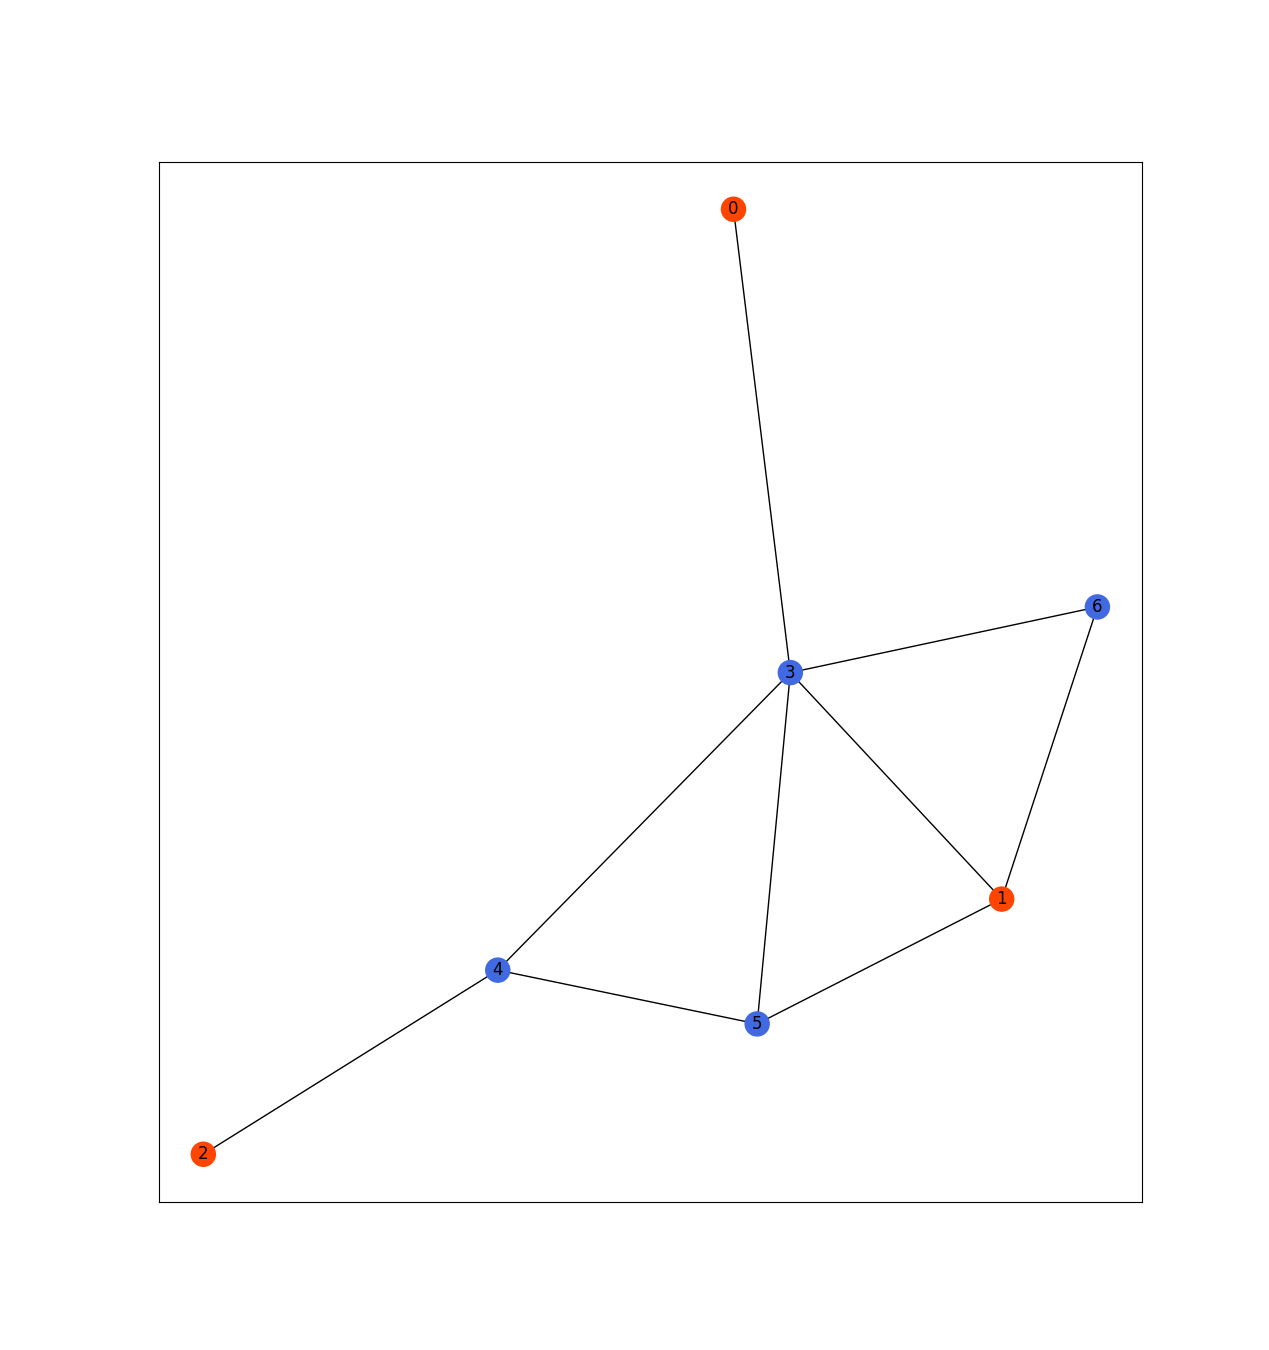
\includegraphics[height=0.7\textheight]{Figure_1.png}
  % \begin{columns}[T] % align columns
  %   \begin{column}{.48\textwidth}
  %   \end{column}%
  %   \hfill%
  %   \begin{column}{.48\textwidth} 
  %   \end{column}%
  % \end{columns}
\end{frame}

\section{Intuitive Approach}
\begin{frame}{Intuitive Approach \trivial}
  \begin{itemize}
    \item Iterate over all vertices
    \item Check if vertex can be added
    \item Complexity: $\mathcal{O}(m)$
    \pause
    \bigskip
    \item Recompute after every update
  \end{itemize} 
\end{frame}

\section{Amortized Complexity}
\begin{frame}
  
\end{frame}

\section{Simple Dynamic Algorithm}
\begin{frame}{Simple Dynamic Algorithm \simple}
  
\end{frame}

\section{Improved Dynamic Algorithm}
\begin{frame}{Improved Dynamic Algorithm}
  \begin{itemize}
    \item Idea: differentiate between \textbf{heavy} and \textbf{light} vertices
    \item $v$ is \textbf{light} if: $deg(v) < m_c$
  \end{itemize}
  \begin{enumerate}
    \pause
    \bigskip
    \item \simple for light vertices
    \medskip
    \item \trivial for heavy vertices
    \begin{itemize}
      \item considering the IS on the light nodes
    \end{itemize}
  \end{enumerate} 
\end{frame}

\begin{frame}{Improved Dynamic Algorithm}
  \begin{itemize}
    \item $m_c := m^{2/3}$
    \item New phase if $m \geq 2m_c \lor m \leq m_c/2$
  \end{itemize}
\end{frame}

\section{Conclusion}
\begin{frame}
  \begin{itemize}
    \item Code and slides at: \\
          \href{https://www.github.com/thilofischer/dynamic_mis}{github.com/thilofischer/dynamic\_mis}
  \end{itemize}
\end{frame}


\end{document}
